Allgemeine Bemerkungen zu Effizienz- und Performancebetrachtungen
Die Effizienz- und Performancebetrachtungen sind stark von der Qualität des Compilers abhängig. Die aktu-elle Version des GNU-Compilers (Version 7.4.0) erzeugt sehr effizienten Code, da die Link-Time Optimiza-tion eingeführt wurde. Im Gegensatz zur Compile-Time Optimization wird der aus den einzelnen Objectfiles gelinkte Programmcode als Ganzes analysiert und optimiert.
Die folgenden Optionen der GNU-Compiler könnten nützlich sein:

\medskip
\noindent
-E \qquad Precompile only, der Output wird auf stdout geschrieben \\
-S \qquad Assembleroutput, ohne Objectfile erzeugen\\
-c \qquad nur compilieren\\
-O0 \qquad keine Optimierung\\
-O1 \qquad Optimierungsstufe 1 (siehe g++ --help für Details)\\
-O2 \qquad Optimierungsstufe 2\\
-O3 \qquad Optimierungsstufe 3\\
-Os \qquad Optimierung auf Codegrösse\\

Hinweise zum x86-Instruktionssatz finden Sie unter anderem im Manual 64-ia-32-architectures-software-developer-manual-325462.pdf und auf folgenden Websites:

\url{http://en.wikipedia.org/wiki/X86_instruction_listings}

\url{http://www.cs.uaf.edu/2005/fall/cs301/support/x86/index.html}

\url{http://ref.x86asm.net/}

\subsection{Aufgabe 1: inline-Methoden}

Bei sehr kurzen Methoden (Einzeiler) ist der Overhead eines Funktionsaufrufs recht gross. Durch Inlining kann der Funktionsaufruf vermieden werden, der Code (Funktionsrumpf) wird vom Compiler direkt anstelle des Funktionsaufrufs gesetzt. Der Compiler wird üblicherweise keinen Inlinecode erzeugen, falls die Funk-tion rekursiv aufgerufen wird oder falls ein Pointer auf diese Funktion verwendet wird. Eine weitere Schwie-rigkeit ergibt sich, wenn die Inlinefunktionen in mehreren Sourcefiles verwendet werden sollen, der Linker kann aus einer bestehenden Objektdatei kaum Inlinecode erzeugen.

Für diese Aufgabe sind zusätzlich die folgenden Optionen der GNU-Compiler nützlich:

\texttt{-Winline} Erzeugt eine Warnung, falls von einer mit inline spezifizierten Funktion kein Inlinecode er-zeugt werden konnte.
Verwenden Sie für diese Untersuchungen die Linux-Konsole im Ubuntu-Image, Eclipse bietet keine Vorteile.

\begin{enumerate}
  \item Wenn bei Klassendeklarationen der Code direkt definiert wird, sind diese Funktionen implizit inline. Ver-wenden Sie den im Verzeichnis ./Vorgabe/Rectangle zur Verfügung gestellte C++-Code. Wie Sie feststellen, ist die Methode getArea() nicht inline. Compilieren Sie dieses Programm, ein Makefile steht zur Verfügung.
  \item Betrachten Sie die erzeugten Assemblerfiles. Welche Methoden sind inline, welche nicht? Hinweis: betrachten Sie dazu die call-Befehle.
  \item Wenn Sie die einzelnen *.s-Dateien betrachten, können Sie nicht feststellen, ob der Linker allenfalls auch noch optimieren kann. Relevant ist einzig, wie der Code in der Programmdatei aussieht. Verwen-den sie den Debugger gdb von der Kommandozeile, um dies festzustellen. Starten Sie die Debugsession mit dem Befehl gdb ./main. Anschliessend müssen Sie das Programm starten mit start. Den disassemblierten Code sehen Sie, wenn Sie disassem eintippen. Im Folgenden sehen Sie den Ausschnitt einer Debugsession.

  \begin{lstlisting}[language=C++, style=C++]
  gdb ./main
    GNU gdb (Ubuntu 8.1-0ubuntu3.2) 8.1.0.20180409-git
    ...
    (gdb) start
    Temporary breakpoint 1 at 0x66e
    ...
    Temporary breakpoint 1, 0x000055555555466e in main ()
    (gdb) disassem
    Dump of assembler code for function main:
      0x000055555555466a <+0>:  push   %rbp
      0x000055555555466b <+1>:  mov    %rsp,%rbp
    => 0x000055555555466e <+4>: sub    $0x40,%rsp
    ...
  \end{lstlisting}


  \item Wahrscheinlich haben Sie festgestellt, dass alle Methoden mit einem Call aufgerufen werden. Ändern Sie die Optimierungsstufe bis alle Methoden ausser getArea() inline sind.
\item Sie möchten nun sowohl die impliziten Inlinefunktionen ins cpp-File zügeln, als auch von getArea() In-linecode erhalten. Sie müssen die Funktionen mit inline kennzeichnen. Häufig werden die Implementa-tionen der Inlinefunktionen direkt unter die Klassendeklaration verschoben.
\item Testen Sie, ob alles richtig funktioniert, indem Sie ein Projekt mit mehreren cpp-Files erstellen, welche die Inlinefunktionen verwenden, d.h. main.cpp plus ein weiteres File. Betrachten Sie die Assemblerfiles, es sollten keine Calls auf Memberfunktionen mehr geben.
\end{enumerate}

\subsubsection{Lösung}

\begin{enumerate}
\item just do it
\item Bei Optimierungsstufe 0 sind keine Funktionen inline (siehe ./Loesung/A1-b). Man erkennt das daran, dass bei den einzelnen Funktionen Labels definiert sind und mit einem Return (\texttt{ret}) abgeschlossen werden. Die Funktionen werden mit einem \texttt{call}-Befehl aufgerufen (siehe folgenden Ausschnitt)

\begin{center}
  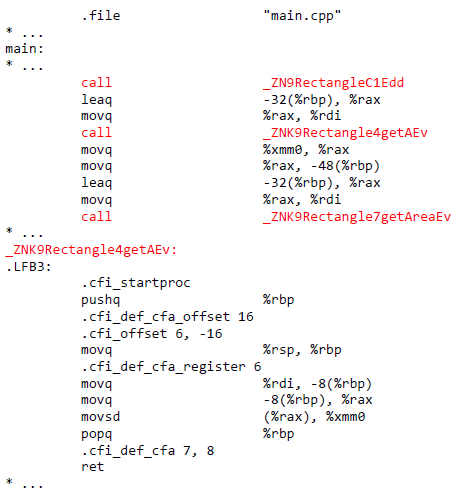
\includegraphics[width=.8\linewidth]{900-Praktika/prak07/1.PNG}
\end{center}

\item Der Debugger-Output zeigt, dass bei Optimierungsstufe 0 alle Funktionen mit call aufgerufen werden.

\begin{center}
  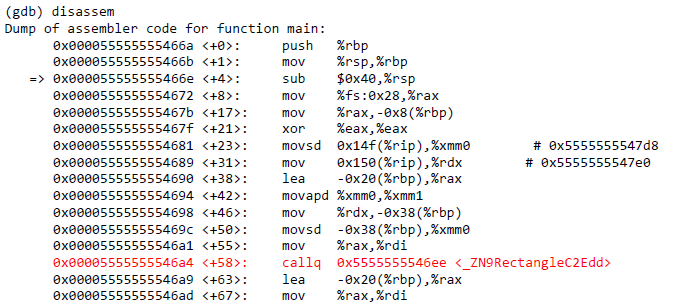
\includegraphics[width=.8\linewidth]{900-Praktika/prak07/2.PNG}
  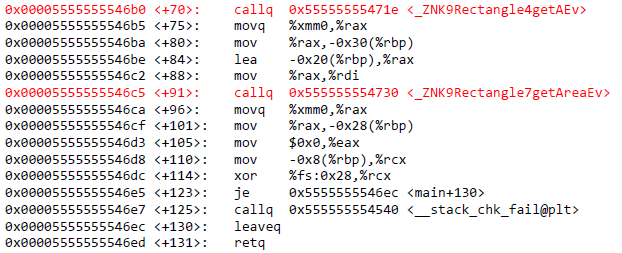
\includegraphics[width=.8\linewidth]{900-Praktika/prak07/3.PNG}

\end{center}

\item Ab Optimierungsstufe 1 sind die impliziten inline-Funktionen alle inline, auch der Konstruktor (siehe Zeile 0x00005555555546a4 $<$+58 $>$: in Aufgabe c). Einzig die Funktion \texttt{getArea()} wird immer noch aufgerufen, da diese Funktion in einer anderen Objectdatei liegt (siehe ./Loesung/A1-d/*.s). Der Assemblerdump zeigt das:

\begin{center}
  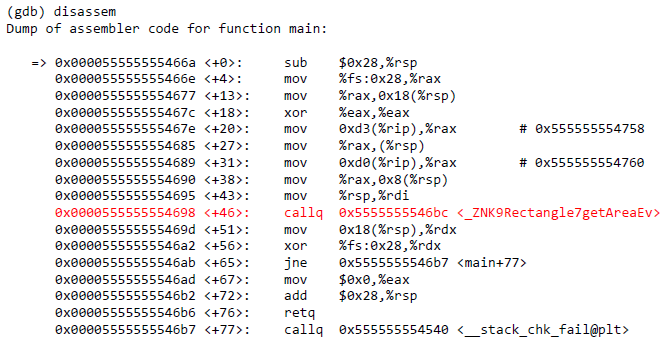
\includegraphics[width=.8\linewidth]{900-Praktika/prak07/4.PNG}
\end{center}

\item Wenn das bestehende \texttt{main()} genommen wird, so optimiert der Compiler ab Optimierungsstufe 1 alle Variablen weg, da sie nicht verwendet werden (siehe ./Loesung/A1-e1/main.s).

\begin{center}
  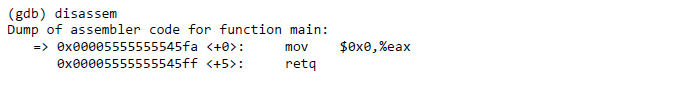
\includegraphics[width=.8\linewidth]{900-Praktika/prak07/7.PNG}
\end{center}


In der beiliegenden Lösung (siehe ./Loesung/A1-e2) werden die Daten deshalb auf cout geschrieben oder die Variablen als volatile deklariert, d.h. die Berechnungen können nicht wegoptimiert werden. Die Methoden können bei der Deklaration, bei der Definition oder bei beiden Stellen mit inline gekenn-zeichnet werden.
\item siehe ./Loesung/A1-f
Eine neue Funktion \texttt{getRectangleB(const Rectangle\& r)} wurde im File rectangleB.cpp eingeführt. Die Funktion verwendet inline Methoden der Rectangle-Klasse um b zu berechnen. Im gdb-Dump kann nachgeprüft werden das im main nur ein einziger Call vorkommt (\texttt{getRectangleB())}:

\begin{center}
  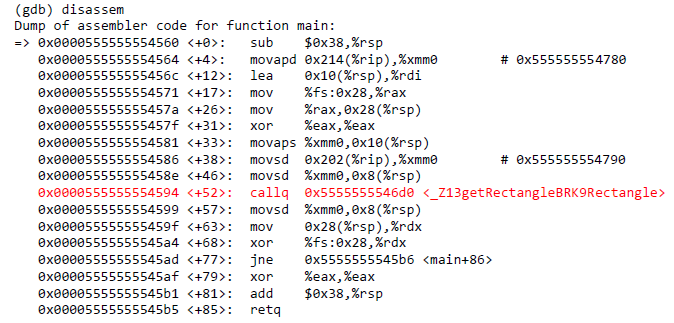
\includegraphics[width=.8\linewidth]{900-Praktika/prak07/5.PNG}
\end{center}


Zudem darf in der Funktion \texttt{getRectangleB()} kein Call vorkommen, da die verwendeten Methoden inline sein müssen:

\begin{center}
  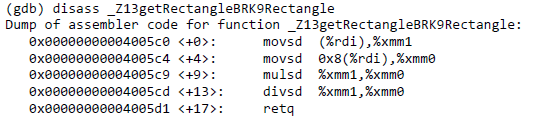
\includegraphics[width=.8\linewidth]{900-Praktika/prak07/6.PNG}
\end{center}

\end{enumerate}

\subsection{Aufgabe 2: Bitfelder}

Gegeben ist das nachfolgende Register

\begin{center}
  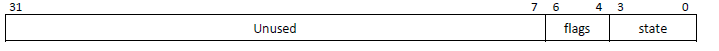
\includegraphics[width=.8\linewidth]{900-Praktika/prak07/bitmuster.PNG}
\end{center}


\begin{enumerate}
  \item Definieren Sie dieses Register mit Hilfe eines Bitfelds. Die Variable (z.B. r) müssen Sie mit volatile kennzeichnen. Wieso?
\item Setzen Sie nun state auf den Wert 15 und flags auf den Wert 3. Untersuchen Sie, wie der Assembler-code aussieht.
\item Inkrementieren Sie nun flags mittels ++r.flags. Achten Sie nun auf den Code.
\item Führen Sie mit flags eine übliche Bitoperation durch, z.B. r.flags \&= 6. Achten Sie nun auf den Code.
\item Diskutieren Sie die erhaltenen Ergebnisse. Entspricht das Resultat Ihren Erwartungen? Worüber sind Sie überrascht? Sollen Bitfelder so verwendet werden? Sollen sie überhaupt verwendet werden?
\end{enumerate}

\subsubsection{Lösung}

\begin{enumerate}
  \item volatile muss verwendet werden, weil die Variable auf ein Hardwareregister gemappt wird und nicht wegoptimiert werden darf. Zudem können die Werte von Registern ebenfalls durch die Hardware geändert werden. Deshalb muss der Code so generiert werden, dass das Register jedesmal zuerst gelesen wird bevor damit gearbeitet wird. Wenn dies nicht gemacht würde, könnte passieren, dass mit einer Ko-pie des Registerinhalts gearbeitet wird, der in der Zwischenzeit durch die Hardware geändert wurde.
  \lstinputlisting[language=C++, style=C++, multicols=2]{900-Praktika/prak07/Loesung/A2/main.s}

\item Die Registervariable wird auf -4(\%ebp) gelegt, d.h. auf den Stack. Aus dem Zugriff auf state wird direkt eine OR-Operation (orl). Da die Variable volatile ist, werden die Werte laufend zwischen dem Stack und dem Register eax hin- und hergeschoben. Der Wert auf dem Stack muss immer der richtige und aktuelle sein.
\begin{lstlisting}[language=C++, style=C++]
movl     $0, -4(%rsp)
...
movl     -4(%rsp), %eax
orl      $15, %eax
movl     %eax, -4(%rsp)
\end{lstlisting}
Das direkte Setzen von flags wird ebenfalls in eine OR-Operation umgewandelt, wobei die flags-Bits zuerst ausmaskiert werden (andl \$-113,\% eax).
\begin{lstlisting}[language=C++, style=C++]
movl    -4(%rsp), %eax
andl    $-113, %eax
orl     $48, %eax
movl    %eax, -4(%rsp)
\end{lstlisting}
\item Beim Inkrementieren von flags wird mit Schiebeoperationen (zuerst nach rechts, dann nach links) und den Registern A und D gearbeitet. Dieser Zugriff wird sehr ineffizient.
\begin{lstlisting}[language=C++, style=C++]
movl       -4(%rsp), %eax
movl       -4(%rsp), %edx
shrl       $4, %eax
addl       $1, %eax
andl       $-113, %edx
andl       $7, %eax
sall       $4, %eax
orl%edx,   %eax
movl       %eax, -4(%rsp)
\end{lstlisting}
\textbf{Pseudocode:}
\begin{enumerate}
  \item  Wert von r in die Register A und D kopieren
    \item Register D um 4 Bits nach rechts schieben, um eins Inkrementieren, mit 7 ausmaskieren und wieder um 4 Bits nach links schieben
    \item Flags-Bits in Register A ausmaskieren und mit Register D verodern
    \item Register A in r speichern
\end{enumerate}
\textbf{Hinweis für den Registerzugriff (Beispiel Register D):}

\begin{lstlisting}[language=C++, style=C++]
|63..32|31..16|15-8|7-0|
               |DH.|DL.| <- DH / DL adressieren das High- / Low-Byte der untern 16
                            Bits von Register D
               |DX.....| <- adressiert die unteren 16 Bits von Register D
       |EDX............| <- EDX adressiert die unteren 32 Bits von Register
|RDX...................| <- RDX adressiert alle 64 Bits von Register D
\end{lstlisting}
\item Auch die Operation r.flags \&= 6 wird sehr ineffizient durchgeführt, da das Muster zuerst an Bitposition 0 geschoben wird, dann wird die Operation durchgeführt und abschliessend wieder zurückgeschoben.
\item Bitfelder sind bekanntlich nicht standardisiert. Wenn die einzelnen Felder direkt gesetzt werden, dann erzeugt der GNU-Compiler effizienten Code, er nimmt direkt eine Bitoperation. Wenn hingegen Operatio-nen durchgeführt werden wie r.flags \&= 6, dann wird sehr ineffizienter Code generiert. Die meisten anderen Compiler können das auch nicht besser. Bitfelder sollten deshalb aus meiner Sicht nicht ver-wendet werden, da nebst der nicht vorhandenen Portabilität zudem sehr ineffizienter Code entsteht.

\end{enumerate}

\subsection{Aufgabe 3: Bitmasken}
\begin{enumerate}
  \item Lösen Sie die Aufgabe 3 mit allen Operationen ausser der Addition direkt mittels (inline-) Operationen mit Bitmasken. Vergleichen Sie nun den Assemblercode mit dem Code aus Aufgabe 3.
\item  Welche Erkenntnisse haben Sie aus den Resultaten der Aufgaben 3 und 4 gewonnen?
\end{enumerate}

\subsubsection{Lösung}

\begin{enumerate}
  \item Bei dieser Variante entsteht sehr effizienter Code. Eine Anweisung wie r \&= 6 $<<$ 4; wird direkt in ein AND umgewandelt, die Operation 6 $<<$ 4 berechnet der Compiler, nicht das Laufzeitsystem:
  lstinputlisting[language=C++, style=C++, multicols=2]{900-Praktika/prak07/Loesung/A3/main.s}
  \begin{lstlisting}[language=C++, style=C++]
movl       $0, -4(%rsp)
movl       $15, -4(%rsp)
movl       -4(%rsp), %eax
orl        $48, %eax
movl       %eax, -4(%rsp)
movl       -4(%rsp), %eax
andl       $96, %eax
movl       %eax, -4(%rsp)
  \end{lstlisting}
  \item  Bitmasken verwenden, Bitfelder nicht.


\end{enumerate}
